\documentclass[tikz,border=8pt]{standalone}

% ---------- Packages ----------
\usepackage[T1]{fontenc}
\usepackage{tikz}
\usetikzlibrary{arrows.meta, shapes, positioning, calc, 
                backgrounds, fit, decorations.pathmorphing, decorations.pathreplacing}

% ---------- Custom Styles ----------
\tikzstyle{imgbox} = [rectangle, rounded corners=2pt, draw=black, fill=gray!15,
  minimum width=2.2cm, minimum height=0.6cm, 
  font=\small\bfseries, align=center, text=black]

\tikzstyle{encblock} = [rectangle, rounded corners=2pt, draw=blue!70!black, fill=blue!20,
  minimum width=2.2cm, minimum height=0.55cm,
  font=\footnotesize, align=center, text=black]

\tikzstyle{diffbox} = [rectangle, rounded corners=2pt, draw=red!70!black, fill=red!15,
  minimum width=2.5cm, minimum height=0.7cm,
  font=\small\bfseries, align=center, text=black]

\tikzstyle{decblock} = [rectangle, rounded corners=2pt, draw=green!60!black, fill=green!15,
  minimum width=2.5cm, minimum height=0.55cm,
  font=\footnotesize, align=center, text=black]

\tikzstyle{outbox} = [rectangle, rounded corners=2pt, draw=orange!70!black, fill=orange!10,
  minimum width=3cm, minimum height=0.7cm,
  font=\small\bfseries, align=center, text=black]

\tikzstyle{lossbox} = [rectangle, rounded corners=2pt, draw=purple!60!black, fill=purple!10,
  minimum width=5cm, minimum height=0.7cm,
  font=\footnotesize, align=center, text=black]

\tikzstyle{arr} = [-{Stealth[length=4pt]}, thick]
\tikzstyle{skip} = [-{Stealth[length=3pt]}, dashed, gray!60, thin]
\tikzstyle{share} = [{Stealth[length=3pt]}-{Stealth[length=3pt]}, 
  thick, red!60!black]

\begin{document}
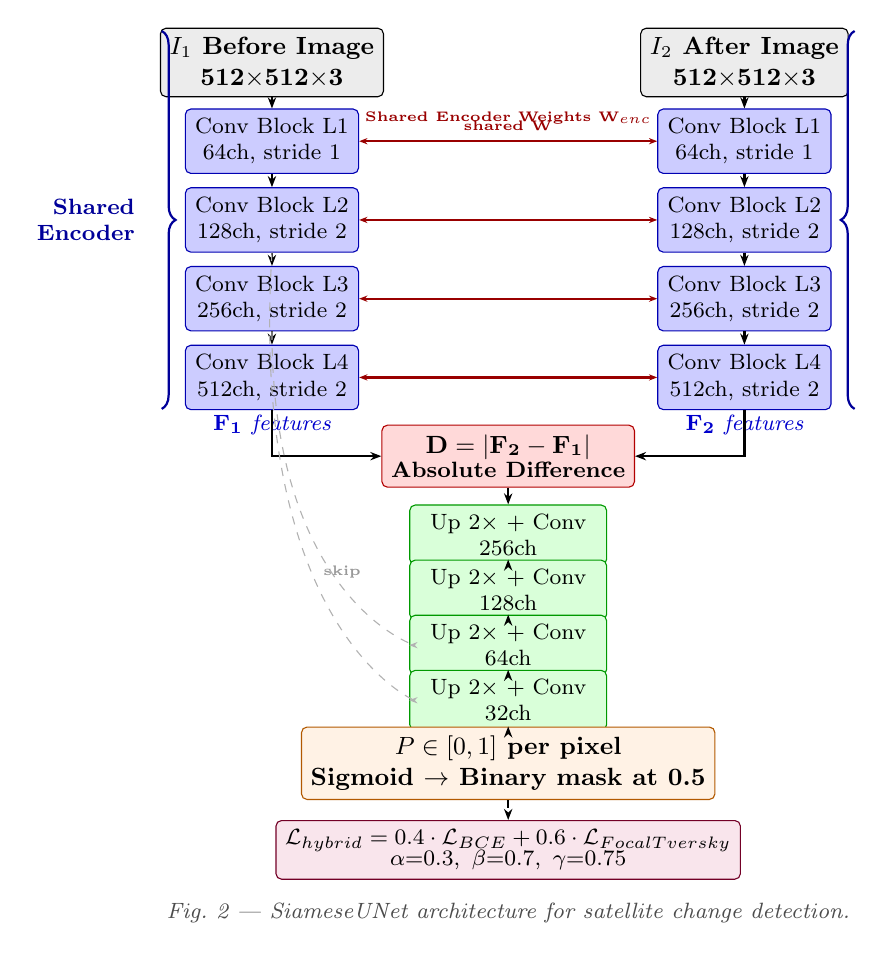
\begin{tikzpicture}[node distance=0.5cm]

  % LEFT BRANCH (Before Image)
  \node[imgbox] (I1) at (-3, 6) {$I_1$ Before Image\\512$\times$512$\times$3};
  
  \node[encblock] (E1a) at (-3, 5) {Conv Block L1\\64ch, stride 1};
  \node[encblock] (E1b) at (-3, 4) {Conv Block L2\\128ch, stride 2};
  \node[encblock] (E1c) at (-3, 3) {Conv Block L3\\256ch, stride 2};
  \node[encblock] (E1d) at (-3, 2) {Conv Block L4\\512ch, stride 2};
  \node[font=\footnotesize\itshape, text=blue!80!black] at (-3, 1.4) {$\mathbf{F_1}$ features};

  \draw[arr] (I1) -- (E1a);
  \draw[arr] (E1a) -- (E1b);
  \draw[arr] (E1b) -- (E1c);
  \draw[arr] (E1c) -- (E1d);

  % RIGHT BRANCH (After Image)
  \node[imgbox] (I2) at (3, 6) {$I_2$ After Image\\512$\times$512$\times$3};
  
  \node[encblock] (E2a) at (3, 5) {Conv Block L1\\64ch, stride 1};
  \node[encblock] (E2b) at (3, 4) {Conv Block L2\\128ch, stride 2};
  \node[encblock] (E2c) at (3, 3) {Conv Block L3\\256ch, stride 2};
  \node[encblock] (E2d) at (3, 2) {Conv Block L4\\512ch, stride 2};
  \node[font=\footnotesize\itshape, text=blue!80!black] at (3, 1.4) {$\mathbf{F_2}$ features};

  \draw[arr] (I2) -- (E2a);
  \draw[arr] (E2a) -- (E2b);
  \draw[arr] (E2b) -- (E2c);
  \draw[arr] (E2c) -- (E2d);

  % SHARED WEIGHT ANNOTATIONS
  \draw[share] (E1a.east) -- node[above, font=\tiny\bfseries, red!60!black] {shared $\mathbf{W}$} (E2a.west);
  \draw[share] (E1b.east) -- (E2b.west);
  \draw[share] (E1c.east) -- (E2c.west);
  \draw[share] (E1d.east) -- (E2d.west);
  
  \node[font=\tiny\bfseries, red!60!black] at (0, 5.3) {Shared Encoder Weights $\mathbf{W}_{\text{enc}}$};

  % DIFFERENCE MODULE
  \node[diffbox] (DIFF) at (0, 1) {$\mathbf{D} = |\mathbf{F_2} - \mathbf{F_1}|$\\[-2pt]\footnotesize Absolute Difference};
  \draw[arr] (E1d.south) |- (DIFF.west);
  \draw[arr] (E2d.south) |- (DIFF.east);

  % DECODER
  \node[decblock] (D1) at (0, 0) {Up 2$\times$ + Conv\\256ch};
  \node[decblock] (D2) at (0,-0.7) {Up 2$\times$ + Conv\\128ch};
  \node[decblock] (D3) at (0,-1.4) {Up 2$\times$ + Conv\\64ch};
  \node[decblock] (D4) at (0,-2.1) {Up 2$\times$ + Conv\\32ch};
  
  \draw[arr] (DIFF) -- (D1);
  \draw[arr] (D1) -- (D2);
  \draw[arr] (D2) -- (D3);
  \draw[arr] (D3) -- (D4);

  % Skip connections from encoder
  \draw[skip] (E1c.south) .. controls (-3,-0.8) and (-1.2,-1.4) .. (D3.west)
    node[midway, above, font=\tiny\bfseries, gray!80] {skip};
  \draw[skip] (E1b.south) .. controls (-3.3,-1.2) and (-1.2,-2.1) .. (D4.west);

  % OUTPUT
  \node[outbox] (OUT) at (0,-2.9) {$P \in [0,1]$ per pixel\\Sigmoid $\rightarrow$ Binary mask at 0.5};
  \draw[arr] (D4) -- (OUT);

  % LOSS FUNCTION BOX
  \node[lossbox] (LOSS) at (0,-4) {$\mathcal{L}_{\text{hybrid}} = 0.4\cdot\mathcal{L}_{\text{BCE}} + 0.6\cdot\mathcal{L}_{\text{FocalTversky}}$\\[-2pt]\footnotesize $\alpha{=}0.3,\ \beta{=}0.7,\ \gamma{=}0.75$};
  \draw[arr, dashed] (OUT) -- (LOSS);

  % Braces around encoders
  \draw[decorate, decoration={brace, amplitude=5pt}, thick, blue!60!black]
    (-4.4, 6.4) -- (-4.4, 1.6) 
    node[midway, left=6pt, font=\footnotesize\bfseries, blue!60!black, align=right] {Shared\\Encoder};
  
  \draw[decorate, decoration={brace, amplitude=5pt, mirror}, thick, blue!60!black]
    (4.4, 6.4) -- (4.4, 1.6);

  % Caption
  \node[font=\footnotesize\itshape, text=black!70] at (0,-4.8) {Fig.~2 --- SiameseUNet architecture for satellite change detection.};

\end{tikzpicture}
\end{document}
